\chapter{Background}\label{chap:background}

Imagine the following task between two players, Anne and Bill. Between Anne and Bill is a lever in the middle position and has five positions in total. Anne thinks the lever should be pulled two positions to her side and Bill thinks the lever should be pulled two positions to his side.
Anne does not know Bill has a goal on his side, and Bill does not know Anne has a goal on her side.
This can be seen in figure \ref{leverexample}.\\
\begin{figure}[h!]
  \begin{centering}
  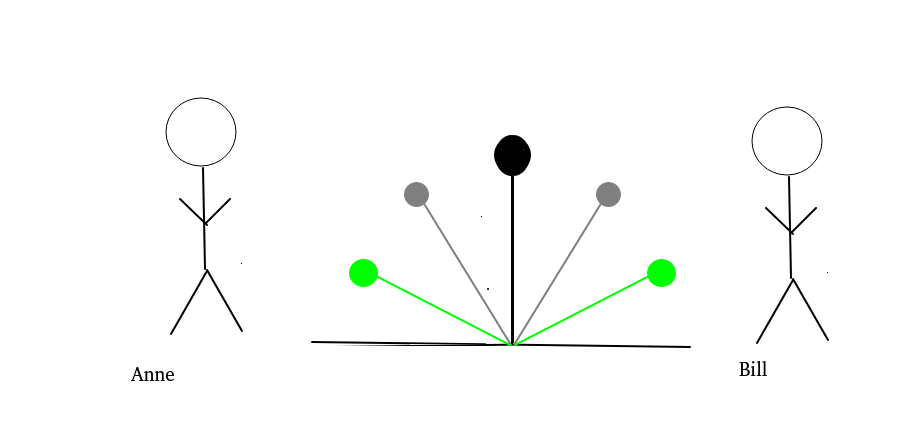
\includegraphics[scale=0.5]{figures/pictures/Hebelbild.png}
  \caption{Visualization of the example}
  \label{leverexample}
  \end{centering}
\end{figure}
 \\

With the asynchronous execution order this task could be easily finished if Anne or Bill just pulled the lever two times in their direction. But just as easily this task could go on a really long time if Anne and Bill pulled the lever alternating, once to the right and then to the left, then to the right again and so on. This could go on infinitely. With no set execution order, how can we prevent the task from going on infinitely? To answer this question we first need to introduce the formal framework.

\section{Dynamic Epistemic Logic}
In the following we will define and explain the core concepts of the Dynamic Epistemic Logic (DEL). DEL is a specific mathematical language used as the framework of this thesis.

The definitions are taken from the work of Bolander et al. \cite{bolander2018better} and \cite{bolander2017gentle} and the book ``Dynamic epistemic logic'' from Ditmarsch \cite{Ditmarsch2007}.

Let $\mathcal{A}$ be a finite set of agents, from the example above this would be $\mathcal{A} =\{$Anne, Bill$\}$. Let $\mathcal{P}$ be a finite set of atomic propositions. Atomic propositions, like $p$ or $q$, describe some affairs that can be true or false.
The epistemic language $\mathcal{L}_{\text{KC}}$ is: \\
$$
\varphi ::= \top \ | \ \bot \ | \ p \ | \ \neg \varphi \ | \ \varphi \wedge \varphi \ | \ K_i \varphi \ | \ C\varphi
$$

with $p \in \mathcal{P}$ and $i \in \mathcal{A}$.
$\top$ describes $\varphi$ as being true, $\bot$ as false.
$K_i \varphi$ reads as ``Agent $i$ knows $\varphi$''. $C \varphi$ reads as ``it is common knowledge that $\varphi$ ''.\\
From the example before, the two agents, $a$ (Anne) and $b$ (Bill) have two goal positions, goal $p$ (lever to the left) and $q$ (lever to the right). Anne knows that one goal position is the left, but does not know the other: $K_a p \wedge \neg K_a q$ . Bill knows that one goal position is the right, but does not know the other position: $\neg K_b  p \wedge K_b q$.


Formulas are evaluated in epistemic models %\todo{not defined}
$$
\mathcal{M}=(W, (\sim_i)_{i \in \mathcal{A}}, V)
$$
with the domain $W$ being a nonempty finite set of worlds,
$\sim_i$ being an equivalence relation called the indistinguishably relation for agent $i \in \mathcal{A}$ and $V : \mathcal{P} \rightarrow \mathcal{P}(W)$ assigning a valuation to each atomic proposition.


Using Anne and Bill as an example, Anne only knows $p$ is true. She does not know if $p \land q$ or $p \land \neg q$, so she sees two worlds. Those two worlds are indistinguishable for Anne. Bill only knows $q$ is true, he does not know if $p \land q$ or $\neg p \land q$. One world where just the lever to the left is a goal, a world where another goal is the lever to the right and a world where just the lever to the right is a goal. Let $w_1$ be the world where just the lever to the left is a goal, $w_2$ be the world where the goal is the lever to the left or to the right and $w_3$ be the world where the goal is the lever to the right. Then $w_1 \sim_\text{Anne} w_2$ and $w_2 \sim_\text{Bill} w_3$. A graphic representation of this would be the global state $s = (\mathcal{M}, w_2)$ with the nodes representing the worlds and the edges representing the indistinguishably relation. The circle around a node represent designated worlds. In all graphic representations in this thesis we usually omit reflexive edges and edges that can be implied by transitivity for better readability.
\[
s=
\begin{tikzpicture}
  \draw (-2,0) node[world, label=below:{$w_1: p, \neg q$}] (w1) {};
  \draw (0,0) node [desig] {}; % designation
  \draw (0,0) node[world, label=below:{$w_2: p,q$}] (w2) {};
  \draw (2,0) node[world, label=below:{$w_3: \neg p, q$}] (w3) {};
  \draw (w1) -- node[above] {Anne} (w2);
  \draw (w2) -- node[above] {Bill} (w3);
\end{tikzpicture}
\]


For $W_d \subseteq W$, the pair $(\mathcal{M}, W_d)$ is called an epistemic state (or simply a state) and the worlds of $W_d$ are called designated worlds. A state is called global if $W_d=\{w\}$ for some world $w$ (called the actual world). We then often write $(\mathcal{M},w)$ instead of $(\mathcal{M},\{w\} )$. We use $S^{gl}(P,\mathcal{A})$ to denote the set of global states (or simply $S^{gl}$ if $P$ and $\mathcal{A}$ are clear from context). For any state $ s=(\mathcal{M}, W_d) $ we let $Globals(s)= \{ (\mathcal{M},w) | w \in W_d \} $.
A state $(\mathcal{M}, W_d)$ is called a local state for agent $i$ if $W_d$ is closed under $\sim _i$ (that is, if $w \in W_d$ and $w \sim _i v $, then $v \in W_d$).
Given a state $s=(\mathcal{M}, W_d)$ the associated local state of agent $i$, denoted $s^i$, is $(\mathcal{M},\{v|v\sim _i w \text{ and } w \in W_d\})$. Going from $s$ to $s^i$ amounts to a \textit{perspective shift} to the local perspective of agent $i$.


In the example above, Anne has the local state $s^{\text{Anne}}=(\mathcal{M},\{w_1,w_2\})$ and Bill has the local state $s^{\text{Bill}}=(\mathcal{M},\{w_2,w_3\})$.


Let $(\mathcal{M}, W_d)$ be a state on $P,\mathcal{A}$ with $\mathcal{M}=(W, (\sim_i)_{i \in \mathcal{A}}, V)$. For $i \in \mathcal{A}$, $p \in P$ and $\varphi, \psi \in \mathcal{L}_{\text{KC}}(P,\mathcal{A})$, we define truth as follows:
\begin{align*}
  &(\mathcal{M}, W_d) \models \varphi
    & &\text{ iff } \qquad
    (\mathcal{M},w)\models \varphi \text{ for all } w \in W_d \\
  &(\mathcal{M}, w) \models p
    & &\text{ iff } \qquad
    w \in V(p) \\
  &(\mathcal{M}, w) \models \neg \varphi
    & &\text{ iff } \qquad
    (\mathcal{M},w) \not\models \varphi \\
  &(\mathcal{M}, w) \models \varphi \wedge \psi
    & &\text{ iff } \qquad
    (\mathcal{M},w) \models \varphi \text{ and } (\mathcal{M},w) \models \psi \\
  &(\mathcal{M}, w) \models K_i \varphi
    & &\text{ iff } \qquad
    (\mathcal{M},v) \models \varphi \text{ for all } v \sim_i w \\
  &(\mathcal{M}, w) \models C \varphi
    & &\text{ iff } \qquad
    (\mathcal{M},v) \models \varphi \text{ for all } v \sim^* w \\
  &(\mathcal{M}, w) \models \top
    & &\text{        } \qquad
    \text{always} \\
  &(\mathcal{M}, w) \models \bot
    & &\text{        } \qquad
    \text{never}
\end{align*}
where $\sim^*$ is the transitive closure of $\bigcup_{i \in \mathcal{A}}\sim_i$.


From the example above, in $(\mathcal{M},w_2)$, $w_2$ is the designated world. In this designated world, Anne still does not know if $q$ is true or not. $(\mathcal{M},w_2) \models \neg K_aq \wedge \neg K_a \neg q$.
Performing a perspective sift on $s=(\mathcal{M},w_2)$ for Anne is $(\mathcal{M},w_2)^{\text{Anne}} =(\mathcal{M},\{w_1,w_2\})$. This perspective shift gives us $(\mathcal{M},\{w_1,w_2\})\not\models q$ and $(\mathcal{M},\{w_1,w_2\})\not\models \neg q$. This way, we can verify the knowledge from the global world for an agent by performing a perspective shift for that agent.


\subsection{Epistemic Actions and Product Updates}

An event model is a 4-tuple $\mathcal{E} = \langle E, (\sim_i)_{i\in \mathcal{A}}, pre, \textit{eff}  \rangle$ where the domain $E$ is a non-empty finite set of events; $\sim_i \subseteq E \times E$ is an equivalence relation called the indistinguishably relation for agent $i$;
$pre:E \rightarrow \mathcal{L}_{KC}$ assigns a precondition to each event;
and $\textit{eff}:E \rightarrow \mathcal{L}_{KC}$ assigns a post condition, or effect to each event.
For all $e\in E$, $\textit{eff}(e)$ is a conjunction of literals, that means atomic propositions and their negations, including $\top$ and $\bot$.\\
For $E_d \subseteq E$, the pair $(\mathcal{E}, E_d)$ is called an epistemic action, or simply action and the events in $E_d$ are called a local action for agent $i$ when $E_d$ is closed under $\sim_i$. \\
Each event of an action represents a different possible outcome.
By using multiple events $e, e' \in E$ that are indistinguishable ($e \sim e' )$, it is possible to model only partially observable actions.\\
If the event model has $E=\{e\}$, we will write $\mathcal{E}=\langle pre(e), \textit{eff}(e)\rangle$.

The product update is used to specify the next state resulting from performing an action in a state.
Let a state $s = (\mathcal{M},W_d)$ and an action $a=(\mathcal{E},E_d)$ be given with $\mathcal{M}=\langle W,(\sim_i)_{i \in \mathcal{A}}, V\rangle $ and $\mathcal{E}=\langle E, (\sim_i)_{i \in \mathcal{A}},pre, \textit{eff} \rangle$
then the product update of $s$ with $a$ is defined as $s \otimes a = ((W',(\sim_i')_{i \in \mathcal{A}}, W_d'))$ where :

 \begin{itemize}
   \item each world is paired up with all applicable events \\
   $W'=\{(w,e)\in W \times E ~|~ \mathcal{M}, w \models pre(e)\};$
   \item new worlds are indistinguishable if the old worlds and the events are indistinguishable \\
   $\sim_i'=\{((w,e),(w',e')) \in W'\times W' ~|~ w \sim_i w' \text{ and } e \sim_i e'\};$
   \item propositions become true if the proposition occurred as a positive literal in the effect of the event or the proposition was satisfied in the world before and did not appear negative in the effect \\
   $V'(p) = \{ (w,e) \in W' ~|~ \textit{eff}(e) \models p \text{ or } (\mathcal{M},w \models p \text{ and } \textit{eff}(e)\not \models \neg p)\};$
   \item worlds are designated if both predecessor world and event are designated. \\
   $W_d' = \{ (w,e) \in W' ~|~ w \in W_d \text{ and } e \in E_d\}$.
 \end{itemize}

$a=(\mathcal{E}, E_d)$ is applicable in $s=(\mathcal{M},W_d)$ if for all $w \in W_d$ there is an event $e \in E_d$ such that $(\mathcal{M},w) \models pre(e)$.

Let us imagine a planning task between Lea and Max. Lea puts two cards face down in front of Max. The goal is that Max picks up the queen. The problem here is that Max does not know where the queen is. \\
Lea has put the queen to the right, so $qR$.

\[
s=
\begin{tikzpicture}
  \draw (-2,0) node[world, label=below:{$w_1: \neg qR$}] (w1) {};
  \draw (0,0) node [desig] {}; % designation
  \draw (0,0) node[world, label=below:{$w_2: qR$}] (w2) {};
  \draw (w1) -- node[above] {Max} (w2);
\end{tikzpicture}
\]

There are two types of actions that could be performed to solve this problem:
\begin{enumerate}
  \item Announcement actions \\
    Lea could tell Max where she put the queen. $\omega(a_{\text{announcement}})=\text{Lea}$

    \[
    \begin{tikzpicture}
      \draw (-2,0) node[world, label=below:{$w_1: \neg qR$}] (w1) {};
      \draw (0,0) node [desig] {}; % designation
      \draw (0,0) node[world, label=below:{$w_2: qR$}] (w2) {};
      \draw (w1) -- node[above] {Max} (w2);
    \end{tikzpicture}
    %
    ~\otimes~
    %
    \begin{tikzpicture}
      \draw (0,0) node [desig] {}; % designation
      \draw (0,0) node[world, label=below:{$e_1: \langle qR, \top \rangle $}] (w1) {};
    \end{tikzpicture}
    %
    ~=~
    %
    \begin{tikzpicture}
      \draw (0,0) node [desig] {};
      \draw (0,0) node[world, label=below:{$(w_2, e_1): qR$}] (w1e1) {};
    \end{tikzpicture}
    \]



  \item Sensing actions \\
    Max could look at the left card, then he knows where the queen is.
    $\omega(a_{\text{sense}})=\text{Max}$

    \[
    \begin{tikzpicture}
      \draw (-2,0) node[world, label=below:{$w_1: \neg qR$}] (w1) {};
      \draw (0,0) node [desig] {}; % designation
      \draw (0,0) node[world, label=below:{$w_2: qR$}] (w2) {};
      \draw (w1) -- node[above] {Max} (w2);
    \end{tikzpicture}
    %
    ~\otimes~
    %
    \begin{tikzpicture}
      \draw (-2,0) node[world, label=below:{$e_1: \langle qR, \top \rangle $}] (e1) {};
      \draw (0,0) node [desig] {}; % designation
      \draw (0,0) node[world, label=below:{$e_2: \langle \neg qR, \top \rangle $}] (e2) {};
    \end{tikzpicture}
    %
    ~=~
    %
    \begin{tikzpicture}
      \draw (-2,0) node[world, label=below:{$w_1: \neg qR$}] (w1) {};
      \draw (0,0) node [desig] {}; % designation
      \draw (0,0) node[world, label=below:{$w_2: qR$}] (w2) {};
    \end{tikzpicture}
    \]

\end{enumerate}



\section{Planning tasks}


A planning task $\Pi = \langle s_0, A, \omega, \gamma \rangle$ consists of a global state $s_0$ called the \textit{initial state}; a finite set of actions A; an owner function $\omega: A \rightarrow \mathcal{A}$; and a \textit{goal formula} $\gamma \in \mathcal{L}_{KC}$.

Consider a version of the lever problem from before. For simplicity, in this example there is only one player and the lever can only be pulled once. The planning task $\langle s_0, \{ a_1 \} , \omega, p \rangle$ consists of the initial state $s_0 = $
\begin{tikzpicture}
  \draw (0,0) node [desig] {}; % designation
  \draw (0,0) node[world, label=below:{$\neg p$}] (w1) {};
\end{tikzpicture}
with the lever being in the upright position. The action $a_1$ =
\begin{tikzpicture}
  \draw (0,0) node [desig] {}; % designation
  \draw (0,0) node[world, label=below:{$e_1: \langle \top, p \rangle $}] (w1) {};
\end{tikzpicture}
has the owner $\omega(a_1) = 1$ (player 1). Everything is fully observable for the agent. The intuitive  solution should prescribe the action $a_1$ to agent 1, pulling the lever to the right.

\[
\begin{tikzpicture}
  \draw (0,0) node [desig] {}; % designation
  \draw (0,0) node[world, label=below:{$w_1: \neg p$}] (w1) {};
\end{tikzpicture}
%
~\otimes~
%
\begin{tikzpicture}
  \draw (0,0) node [desig] {}; % designation
  \draw (0,0) node[world, label=below:{$e_1: \langle \top, p \rangle $}] (w1) {};
\end{tikzpicture}
%
~=~
%
\begin{tikzpicture}
  \draw (0,0) node [desig] {};
  \draw (0,0) node[world, label=below:{$(w_1, e_1): p$}] (w1e1) {};
\end{tikzpicture}
\]


A policy $\pi$ for $\Pi = \langle s_0, A, \omega, \gamma \rangle$ is a partial mapping $\pi: S^{gl} \hookrightarrow \mathcal{P}(A)$ such that:
\begin{enumerate}
  \item Applicability\\
    We require actions to be applicable in all states they are assigned to: \\
    for all $a \in S^{gl}, a \in \pi(s): a$ is applicable in $s$.
  \item Uniformity \\
    If the policy $\pi$ prescribes some action $a$ to agent $i$ in state $s$ and agent $i$ cannot distinguish $s$ from some other state $t$, then $\pi$ has to prescribe the same action $a$ for $i$ in $t$ as well: \\
    for all $s,t \in S^{gl} $ such that $ s^{\omega(a)} = t^{\omega(a)}, a \in \pi(s): a \in \pi(t)$

    A planning task with the agents Lea and Max,
    initial state Lea puts two cards face down on the table, one of them is a queen, the other a king. Max does not know if the queen is on the left or the right side. The goal is that Max turns over the queen. Max has two actions, he can either turn over the left card or the right card. The policy in which Max turns over the left card is a valid policy because even though he does not know if that card is the queen, the action is prescribed in both cases.


  \item Determinism \\
    We require $\pi$ to be unambiguous for all agents in the sense that in each state $s$ where an agent $i$ is supposed to act according to $\pi$, $\pi$ will always prescribe the same action for agent $i$.
\end{enumerate}

The properties uniformity and applicability together imply knowledge of preconditions, the property that in each state, an agent who is supposed to perform a particular action must also know that the action is applicable in that state.

We also must allow policies to sometimes prescribe multiple actions of different owners to the same state. This is because the set of indistinguishable states can differ between the agents. To characterize the different outcomes of agents acting according to a common policy, we define the notion of policy executions.

An execution of a policy $\pi$ from a global state $s_0$ is a maximal (finite or infinite) sequence of alternating global states and actions $(s_0, a_1, s_1, a_2, s_2,...)$, such that for all $ m \leq 0$
\begin{enumerate}
  \item $a_{m+1} \in \pi(s_m)$ and
  \item $s_{m+1} \in Globals(s_m \otimes a_{m+1})$
\end{enumerate}
An execution is called successful for a planning task $\Pi = \langle s_0, A, \omega, \gamma \rangle$, if it is a finite execution $(s_0, a_1, s_1,...,a_n, s_n)$ such that $s_n \models \gamma$.

%\extend{Example: Anna lets Bill pull the lever to the right. Globally this makes sense, since that is Bills goal. But individually, this makes no sense at all because Anne doesent know Bills goal.}

In the lever example, a policy could be that, starting in the position with the lever being in the middle, Bill pulls the lever to the right and then to the right again. This is a policy that satisfies all properties and where the last state satisfies the goal formula. The execution of the policy is finite and successful. \\
For Bill, this is a reasonable policy. It satisfies the goal formula he knows to be true, with the lever being at the far right position. But for Anne, it is not a reasonable policy because she can not see that the execution of this policy will satisfy the goal formula.

%\todo{Geht das hier etwas schöner?}
We now want to restrict our focus to policies that are guaranteed to achieve the goal after a finite number of steps. More formally, all of their executions must be successful. As in nondeterministic planning, such policies are called strong (Cimatti et al. \cite{cimattietal}).
For a planning task $\Pi = \langle s_0, A, \omega, \gamma \rangle$, a policy $\pi$ is called strong if $s_0 \in \text{Dom}(\pi) \cup \{s \in S^{gl} ~|~ s \models \gamma\}$ and for each $s \in \text{Dom}(\pi)$, any execution of $\pi$ from $s$ is successful for $\Pi$. A planning task is called solvable if a strong policy for $\Pi$ exists.
For $ i \in \mathcal{A} $ , we call a policy $i$-strong if it is strong and  $Globals(s_0^i ) \subseteq \text{Dom}(\pi) \cup\{ s \in S^{gl} ~|~ s \models \gamma \}$.

When a policy is i-strong it means that the policy is strong and defined on all the global states that agent $i$ cannot distinguish inbetween. It follows directly from the definition that any execution of an $i$-strong policy from any of those initially indistinguishable states will be successful. So if agent $i$ comes up with an $i$-strong policy, agent $i$ knows the policy to be successful.

The policy from above, with Bill pulling the lever to the right twice is Bill-strong but not Anne-strong.

Sometimes the agents cannot coordinate their plans but rather have to come up with plans individually. These plans can differ a lot, the agents often have different knowledge about the states, the actions and therefore the action outcomes. For this reason we will define a policy profile for a planning task $\Pi$ to be a family $(\pi_i)_{i \in \mathcal{A}}$ where each $\pi_i$ is a policy for $\Pi$. We assume actions to be instantaneous and executed asynchronously. This leads to the following generalization:

An execution of a policy profile $(\pi_i)_{i \in \mathcal{A}}$ is a maximal (finite or infinite) sequence of alternating global states and actions $(s_0, a_1, s_1,...)$, such that for all $m \leq 0$,
\begin{enumerate}
  \item $a_{m+1} \in \pi_i(s_m)$ where $i=\omega(a_{m+1})$ \\
    Note here the source of nondeterminism as a result from the possibility of multiple policies prescribing actions for their respective agents.
  \item $s_{m+1} \in Globals(s_m \otimes a_{m+1}) $ \\
    Here the source of nondeterminism is from the possibility of nondeterministic action outcomes.
\end{enumerate}


If all agents have one strong policy in common which all of them follow, then at execution time, the goal is guaranteed to be eventually reached. If, however, each agent acts on its individual strong policy, then the incompatibility of the individual policies may prevent the agents from reaching the goal, even though each individual policy is strong.



The cost of a policy can be defined as its worst-case execution length, the number of actions in its longest possible execution. An optimal policy is one with minimal costs. Due to partial observability and different knowledge, the agents might assign different costs to the same policy and therefore the costs are subjective. \\
Let $\pi$ be a strong policy for a planning task $\Pi$. The perspective-sensitive cost (or simply cost) of $\pi$ from a state $s\in Dom(\pi)$, denoted $\kappa_{\pi}(s)$ is defined as:
$$\kappa_{\pi}(s) =
\begin{cases}
0 \qquad & \text{if there exists no } a \in \pi(s)\\
1+ \max_{a\in \pi(s), s'\in Globals(s^{\omega(a)} \otimes a)} \kappa_{\pi}(s') \qquad & \text{else.}
\end{cases}$$
